\documentclass[11pt,a4paper,appendixprefix=true,numbers=noenddot]{scrreprt}

\usepackage[hidelinks, bookmarks]{hyperref}
\usepackage[utf8]{inputenc}
\usepackage[italian]{babel}
\usepackage{minted}
\usepackage{amsmath, amsfonts}
\usepackage{graphicx}

\usepackage{parskip}
\usepackage{color}

\usepackage{placeins}

\usepackage{algpseudocode}
\usepackage{framed}


\usepackage{url}

\newtheorem{teorema}{Teorema}
\newtheorem{lemma}[teorema]{Lemma}
\newtheorem{proposizione}[teorema]{Proposizione}
\newtheorem{proprieta}[teorema]{Proprietà}

\newcommand{\shellcmd}[1]{\\\indent\indent\texttt{\footnotesize\# #1}\\}

\author{L. De Sano, A. Donizetti}
\title{\textsc{FIC}: Fractal Image Compression}
\date{Settembre 2015}

\begin{document}
\maketitle

\tableofcontents

\chapter{Introduzione}

Con il termine ``Fractal image Compression'' si va ad indicare una famiglia di tecniche di compressione di immagini (o video) basate sulle proprietà matematiche dei frattali. Tali metodi di compressione si rivelano sopra ogni altra cosa adatti a comprimere textures e immagini naturali, o, più in generale, immagini che sono caratterizzate da un elevato livello di \emph{self-similarity} (ovvero aventi delle parti che, al netto di rotazioni e ingrandimenti/riduzioni, somigliano ad altre parti dell'immagine).

La compressione di immagini tramite frattali (così come altre, più diffuse, ad esempio \textit{JPEG}) appartiene a quel gruppo di tecniche di compressione \emph{lossy}, ovvero in cui la compressione dell'immagine avviene al costo di una perdita di informazione. Tuttavia, a differenza di quanto accade quando si utilizza uno dei metodi di compressione basati sui pixel (come \textit{JPEG}, \textit{GIF} o \textit{MPEG}), nella compressione frattale nessuna parte dell'immagine viene effettivamente memorizzata. Ciò che viene memorizzato è invece la \emph{struttura interna} dell'immagine (ad esempio un indice di quali parti, effettuate le dovute trasformazioni, sono simili ad altre parti). 

Poiché nessun pixel dell'immagine originale viene memorizzato, la decompressione parte da un singolo pixel, di colore qualsiasi, e procede alla ricostruzione dell'immagine originale applicando iterativamente una mappa ricavata dalla struttura interna dell'immagine originale.

In questo documento tratteremo delle tecniche di compressione di immagini basate su frattali, iniziando con una panoramica teorica del loro funzionamento, proseguendo con la discussione di alcuni aspetti pratici e presentando una implementazione giocattolo realizzata in MATLAB, e concludendo infine con alcuni test che consentiranno di valutare praticità e \emph{performances} di una libreria di compressione basata su frattali, anche in confronto con altre tecniche di compressione \emph{lossy} maggiormente utilizzate.

\chapter{Aspetti teorici}

\section{Introduzione ai frattali}

Un frattale è un oggetto geometrico che si ripete nella sua forma, allo stesso modo, su diverse scale. Questo comportamento fa si che ingrandendo una sua qualsiasi componente, ciò che si ottiene è una figura simile all'originale. In linea di massima, si può dire che perché l'insieme $F$ sia considerato un frattale, $F$ dovrebbe avere almeno le seguenti proprietà:

\begin{itemize}
\item $F$ ha dettagli ad ogni scala d'ingrandimento;
\item $F$ gode di autosimilitudine (a qualunque scala si osservi, presenta sempre le stesse caratteristiche globali);
\item la dimensione frattale\footnote{La dimensione frattale è un rapporto che fornisce un indice statistico relativo a come varia la complessità di un frattale rispetto alla scala a cui viene misurato.} di $F$ è maggiore della sua dimensione topologica\footnote{La dimensione topologica è un concetto di dimensione che si applica ad uno spazio topologico, ad esempio in $\mathbb{R}^n$ è $n$.};
\item esiste un algoritmo relativamente semplice per costruire $F$.
\end{itemize}

Un esempio di oggetto geometrico secondo i principi di costruzione di un frattale e che rispetta le proprietà elencate è la curva di \textit{Koch}. La costruzione comincia con una linea di lunghezza $1$ chiamata \textit{initiatior}. Da questa linea si rimuove il terzo centrale e lo si sostituisce con due linee della stessa lunghezza della parte rimossa. Questa nuova forma viene chiamata \textit{generator}. La prima parte della costruzione è mostrata in figura \ref{fig:k1}.

\begin{figure}[!ht]
\centering
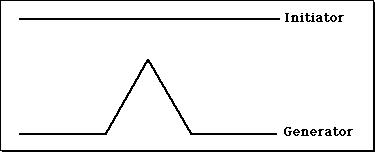
\includegraphics[scale=0.55]{images/koch1.png}
\caption{Initiator e generator per la curva di Koch}
\label{fig:k1}
\end{figure}

La regola può essere nuovamente applicata su ogni linea, così da andare a sostituirla ogni volta come fanno nel passaggio da \textit{initiator} a \textit{generator}. Il secondo livello è visibile in figura \ref{fig:k2}.

\begin{figure}[!ht]
\centering
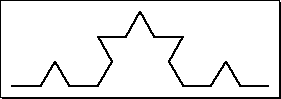
\includegraphics[scale=0.55]{images/koch2.png}
\caption{Livello 2 per la curva di Koch}
\label{fig:k2}
\end{figure}

\FloatBarrier

Una volta che la procedura è avviata può proseguire a piacimento. Il terzo e il quarto livello sono visibili nelle figure \ref{fig:k3} e \ref{fig:k4} rispettivamente.

\begin{figure}[!ht]
\centering
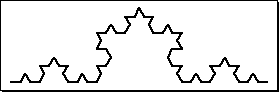
\includegraphics[scale=0.55]{images/koch3.png}
\caption{Livello 3 per la curva di Koch}
\label{fig:k3}
\end{figure}

\begin{figure}[!ht]
\centering
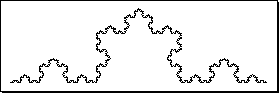
\includegraphics[scale=0.55]{images/koch4.png}
\caption{Livello 4 per la curva di Koch}
\label{fig:k4}
\end{figure}



\section{Iterated Function Systems}

Uno strumento matematico che si rivelerà fondamentale nella fase di decompressione delle immagini trattate con un metodo di compressione frattale è quello degli \emph{Iterated Function Systems}, che andiamo per questo motivo a descrivere qui.

Senza eccedere in formalità, definiamo un \emph{Iterated Function System} (IFS) come una collezione di trasformazioni contrattive $\{w_i : \mathbb{R}^2 \rightarrow \mathbb{R}^2 \}_{i=1,\ldots, n}$ che mappa il piano su se stesso. Questa collezione di trasformazioni definisce una mappa 

\[
W(\cdot) = \bigcup_{i=1}^{n} w_i(\cdot)
\]

Tale mappa è applicata ad insiemi di punti, ed il risultato è definito in questa maniera: dato un insieme di punti $S \in \mathbb{R}^2$, calcoliamo $w_i(S)$ per ogni $i$ (ovvero produciamo $i$ copie ridotte di $S$), e poi calcoliamo l'unione dei risultati (ovvero, mettiamo insieme tutte le copie ridotte), ottenendo così un nuovo insieme $S' = W(S)$.

$W$ così definito è una mappa tra sottoinsiemi di $\mathbb{R}^2$ (che d'ora in avanti per noi saranno ``immagini''), e gode di due importanti (e rilevanti per la compressione frattale) proprietà, che andiamo ad enunciare senza dimostrazione.

\begin{proprieta}
Se tutte le $w_i$ sono contrattive, allora $W$ è contrattiva in uno spazio di sottoinsiemi del piano.
\end{proprieta}

\begin{proprieta}
Fissata una mappa $W$, esiste una immagine $x_W$, chiamata \emph{attrattore per $W$}, tale che
\begin{itemize}
\item $W(x_W) = x_W$
\item data una qualunque immagine di partenza $S_0$, vale che 
\[x_W \equiv \lim_{n \rightarrow \infty} W^{n}(S_0) \]
ovvero l'applicazione ripetuta per $n$ volte di $W$ porta ad ottenere $x_W$, per $n$ sufficientemente grande, ed indipendentemente dalla scelta dell'immagine di partenza.
\item $x_W$ è unica. Se una qualsiasi immagine $S$ soddisfa $W(S) = S$, allora $S$ è l'attrattore per $W$.
\end{itemize}
\end{proprieta}

La seconda di queste proprietà è nota come \emph{Contractive Mapping Fixed-Point Theorem}.

\section{Self-similarity nelle immagini}

\subsection*{Immagini come oggetti matematici}

Per poter applicare la teoria degli \emph{IFS} alle immagini come comunemente le intendiamo (ovvero, in sostanza, matrici di pixels rappresentati  da 1 byte -- \emph{greyscale} -- oppure più di uno -- es. RBG --), è necessario formalizzare in qualche modo il concetto di ``immagine digitale'', cercando di inserirlo in un contesto matematico che ci consenta di manipolarla utilizzando di strumenti messi a disposizione dall'algebra. Per semplicità, ci limiteremo qui a considerare le immagini in \emph{grayscale} (un singolo canale di colore, l'intensità indicata con un numero da 0 a 255).

Consideriamo un'immagine in scala di grigi, memorizzata come matrice di pixel, 1 byte per ogni pixel. Non è difficile immaginare di poter rappresentare tale immagine utilizzando una funzione $f: \mathbb{R}^2 \rightarrow  \{1, 2, \ldots, 255 \}$, in modo tale che ad ogni pixel alle coordinate $(x, y)$ sia fatto corrispondere un punto $(x, y)$ nel piano, al quale a sua volta viene associata un'altezza $z$, che corrisponde al valore di grigio del pixel in questione. 

Ad esempio, ad un'immagine con il primo pixel in basso a sinistra avente livello di grigio 177, viene fatta corrispondere una funzione $f$ che, per quanto riguarda quel preciso punto, avrà $f(0,0) = 177$. Effettuando questa operazione su tutti i pixel dell'immagine originale, è possibile definire completamente $f$ su tutta la parte del piano di nostro interesse (e, in genere, si riduce per convenzione l'immagine ad avere dominio 
$[0, 1]^2$). Nella figura qui sotto riportata si può vedere un esempio del risultato finale della procedura, applicata ad una immagine grayscale $128 \times 128$ pixels.

\begin{figure}[!ht]
\centering
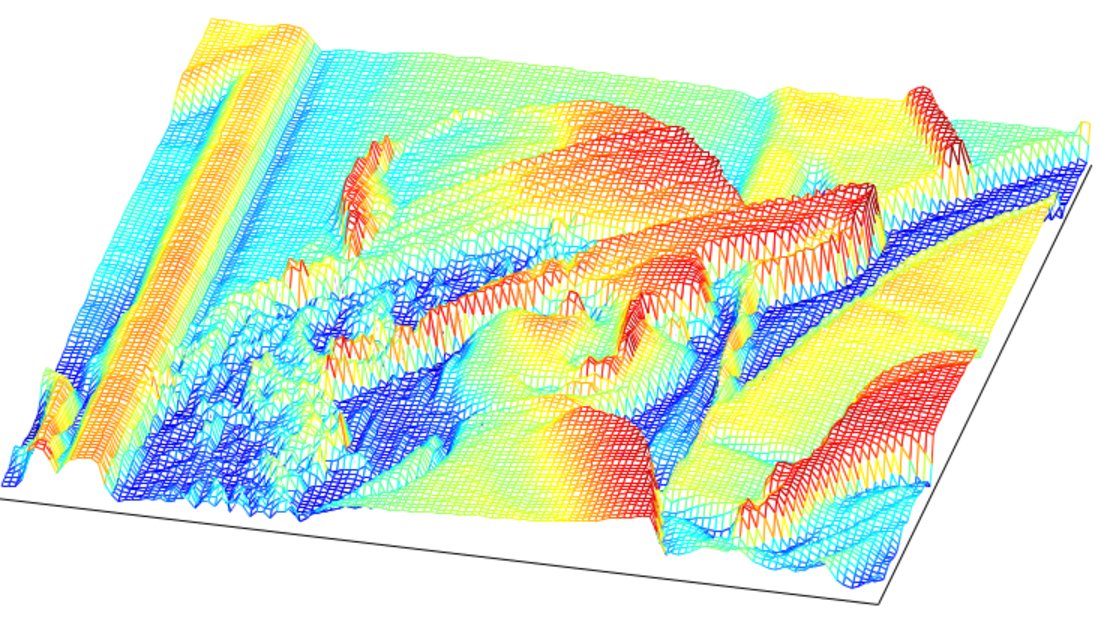
\includegraphics[scale=0.6]{images/lena-mash.pdf} 
\caption{lena grayscale, $128 \times 128$ pixels, trasformata in funzione $[0,1]^2 \rightarrow \{0,\ldots,255 \}$}
\end{figure}

La trasformazione descritta ci permette di ignorare l'aspetto ``visivo'' della modalità in cui una immagine è memorizzata, e ci consente di identificare una immagine con la funzione $f$ associata, su cui si andrà ad operare durante il procedimento di compressione.

\subsection*{Distanza tra due immagini}

Un secondo concetto che è necessario introdurre per poter operare sulle immagini durante il procedimento di compressione e decompressione è quello di ``distanza'' tra due immagini. La contrattività di una mappa $W$ (ovvero, intuitivamente, il fatto che essa rende le immagini più ``piccole'') può essere verificata solo se si ha a disposizione una qualche metrica sulla base della quale è possibile valutare la distanza tra due sottoinsiemi del piano (ovvero, nel nostro caso, due immagini).

Date due immagini $f, g$, definiamo la loro distanza $d(f, g)$, utilizzando la media quadratica, come

\[
d(f,s) = \sqrt{\int_{[0,1]^2} f(x,y) - g(x,y) \quad \text{d}x\text{d}y }
\]

La metrica ci fornisce una maniera di valutare la distanza tra due immagini pesando in maniera uniforme tutti i punti in esse contenuti.

\subsection*{Self-similarity debole}

A differenza di quanto accade quando si osserva un frattale vero e proprio, all'interno di immagini ``naturali'' non troviamo una \emph{self-similarity} forte: solitamente non abbiamo parti dell'immagine che sono simili all'immagine complessiva, bensì parti dell'immagine che sono simili ad altre parti dell'immagine. Un altro aspetto da considerare è quello della colorazione: due parti dell'immagine potrebbero essere simili nella composizione dei pixel, ma differenti per quanto riguarda la gradazione di grigio dei pixels che le compongono. 

I basilari IFS che abbiamo descritto in precedenza vanno leggermente complicati, nel contesto della compressione frattale delle immagini, in modo da accomodare i due aspetti qui sopra descritti. Come prima cosa, notiamo che al momento di definire le trasformazioni $w_i$, dovremo fare in modo che ad ogni trasformazione sia consentito di andare a toccare solo un particolare sottoinsieme del piano, in maniera da accomodare il requisito di poter rappresentare la \emph{self-similarity} debole (similarità tra parti e altre parti, e non con l'intera immagine). Come seconda cosa, alle mappe vanno aggiunti due parametri, \emph{contrasto} e \emph{luminosità}, che ci consentiranno di definire non solo trasformazioni  \emph{spaziali}, ma anche trasformazioni che vanno a coinvolgere la differenza di \emph{colorazione} (sempre su scala di grigi) tra due sottoinsiemi di piano.

Invece della classica trasformazione su $\mathbb{R}^2$ che ci aspetteremmo considerato il fatto che stiamo operando su funzioni $\mathbb{R}^2 \rightarrow \mathbb{R}$, definiamo le $w_i$ come trasformazioni su $\mathbb{R}^3$:

\[
w_i \begin{bmatrix} 
x \\
y \\
z
\end{bmatrix} = \begin{bmatrix}
a_i & b_i & 0 \\
c_i & d_i & 0 \\
0 & 0 & s_i \\
\end{bmatrix} \cdot \begin{bmatrix} 
x \\
y \\
z
\end{bmatrix} + \begin{bmatrix} 
e_i \\
f_i \\
o_i
\end{bmatrix}
\]

La trasformazione è formata da una componente \emph{spaziale}, ovvero

\[
v_i \begin{bmatrix} 
x \\
y \\
\end{bmatrix} = \begin{bmatrix}
a_i & b_i \\
c_i & d_i \\
\end{bmatrix} \cdot \begin{bmatrix} 
x \\
y \\
\end{bmatrix} + \begin{bmatrix} 
e_i \\
f_i \\
\end{bmatrix}
\]

e di due parametri aggiuntivi $s_i$ ed $o_i$, che agiscono rispettivamente come moltiplicatore e scala tramite somma sulla componente $z$ della funzione. Questi due parametri, che chiamiamo rispettivamente \emph{contrasto} e \emph{luminosità}, non influenzano in alcun modo le componenti spaziali della trasformazione, e ci consentono di definire trasformazioni sullo spazio di \emph{colore} dell'immagine (che, ricordiamo, è rappresentato nella funzione associata all'immagine come la componente $z$). 

Ricordando che l'immagine è rappresentata da una funzione $z = f(x,y)$, dove $x$ ed $y$ sono pixels e $z$ il grado di grigio dell'immagine \emph{grayscale}, una singola trasformazione $w_i$ viene applicata calcolando $w_i(f) = w_i(x, y, f(x,y))$. La parte spaziale di $w_i$ determina come una sotto-parte dell'immagine è mappata su altre sottoparti, mentre $s_i$ ed $o_i$ determinano contrasto e luminosità della trasformazione.

Il fatto che il mapping sia da effettuarsi da sottoinsiemi a sottoinsiemi dell'immagine è permesso dal fatto che le varie $w_i$ sono implicitamente definite in modo da operare su un sottoinsieme di $[0,1]^2$, che chiamiamo $D_i$, dando come risultato un sottoinsieme di $[0,1]^2$, che chiameremo $R_i$. In simboli, scriviamo che

\[
v_i(D_i) = R_i
\]

ovvero la componente spaziale della trasformazione ha dominio in sottoinsiemi del piano che chiamiamo $D_i$ e codominio in sottoinsiemi del piano che chiamiamo $R_i$.

Poiché richiediamo che $W(f)$, l'unione delle $w_i$, sia a sua volta un'immagine compatta, le trasformazioni devono soddisfare due proprietà basilari: prima di tutto gli $R_i$ devono partizionare completamente $[0,1]^2$, ovvero deve valere $\bigcup_i R_i = [0,1]^2$. Inoltre gli $R_i$ non devono sovrapporsi, ovvero deve valere $R_i \not= R_j$ se $i \not= j$. Queste due proprietà garantiscono che l'applicazione della mappa $W$ su una immagine $S$ risulti in una immagine $S'$, possibilmente differente, ma completa ed univoca.

Poiché la mappa $W$ è contrattiva solo se lo sono le trasformazioni $w_i$, è necessario scegliere accuratamente i parametri di queste ultime. Dato che la metrica di distanza $d$ che abbiamo definito sopra non prende in considerazione le direzioni $x$ ed $y$, ma soltanto la direzione $z$, per assicurare la contrattività delle $w_i$ è sufficiente fare attenzione al parametro di scala $s_i$. In particolare:

\begin{proprieta}
Le trasformazioni $w_i$ sono contrattive per $s_i < 1$
\end{proprieta}

\subsection*{Decoding}

A questo punto abbiamo tutti gli strumenti che servono per effettuare il \emph{decoding} di una immagine compressa utilizzando frattali: partendo  da una immagine qualunque, si applica ripetutamente la mappa $W$ fino a quando non si raggiunge il suo punto fisso $x_W$, che rappresenta il risultato dell'operazione di decodifica.

L'aspetto interessante (e complicato) della tecnica di compressione che stiamo descrivendo è però un altro: come fare, data una immagine $f$ da comprimere, a trovare un insieme di mappe $\{w_i\}_i$ tale che $f$ sia il punto fisso della loro unione ($W$)? Questa operazione, che rappresenta il nucleo delle tecniche di compressione tramite frattali, è l'argomento della prossima sezione.

\section{Encoding}

Come anticipato nella precedente sezione, per comprimere un'immagine $f$ è necessario trovare una mappa $W$ tale che 

\[
f = W(f)
\]

ovvero una mappa $W$ avente $f$ come attrattore. Ricordando la definizione di $W$, la proprietà richiesta diventa

\[
f = w_1(f) \cup w_2(f) \cup \dots \cup w_N(f)
\]

Per ottenere questo, dovremmo procedere con il partizionare l'immagine $f$ in tanti pezzi tali per cui, applicando le trasformazioni $\{w_i\}_i$, si otterrebbe l'immagine di partenza. Chiaramente, in generale, questa è una condizione troppo restrittiva: ottenere \emph{esattamente} l'immagine di partenza non è qualcosa che sia possibile sperare (a parte nei casi in cui si stia cercando di comprimere un'immagine frattale!).

Quello che facciamo in pratica è cercare delle trasformazioni che, applicate, ci restituiscano un'immagine \emph{differente}, diciamo $f'$, tale per cui la distanza con l'immagine di partenza, ovvero $d(f,f')$, è piccola. Operativamente, procediamo calcolando le $w_i$ con l'obbiettivo di minimizzare la distanza tra il pezzo di immagine che stiamo attualmente considerando e il pezzo di immagine ottenuto dopo l'applicazione della trasformazione. In formula, minimizziamo

\[
d\big(f \cap (R_i \times I), w_i(f)\big) 
\]

per tutti gli $i$. In termini di $R_i$ ed $D_i$ (i concreti pezzi di immagini su cui andremo ad operare), dobbiamo partizionare l'immagine $f$ in una collezione di pezzi $R_i$, e cercare da una seconda collezione $D_i$ dei pezzi tali per cui la mappa da $D_i$ ad $R_i$ comporta un errore (calcolato come distanza $d$) che sia piccolo.

\subsection*{Metrica}

Come abbiamo visto prima la comparazione tra le due immagini avviene tramite la radice della media quadratica. Usare questa metrica ci consente di calcolare i valori ottimali per $s_i$ e di $o_i$ in maniera semplice. In particolare dati due quadrati contenenti $n$ valori di luminosità dei pixel $ai, \dots, a_n$ per $D_i$ e $b_1, \dots, b_n$ per $R_i$, possiamo cercare i valori di $s$ e di $o$ che minimizzano la quantità:

\[
R = \sum_{i=1}^{n}{\left( s \cdot a_i + o - b_i \right) }
\]

Questa quantità ci fornisce i valori di contrasto e luminosità che fanno si che la trasformazione dai i valori di $a_i$  a quelli di $b_i$ abbia la minima distanza possibile. Il valore minimo di $R$ si ha quando le derivate parziali di $s$ e di $o$ si azzerano e questa condizione si ha quando:

\[
s = \dfrac{\left[ n \sum\limits_{i=1}^{n}{a_i b_i} - \sum\limits_{i=1}^{n}{a_i} \sum\limits_{i=1}^{n}{b_i} \right] }
{\left[ n \sum\limits_{i=1}^{n}{a_i^2} - {\left( \sum\limits_{i=1}^{n}{a_i} \right)}^2 \right] }
\]

e

\[
o = \frac{1}{n} \left[ \sum\limits_{i=1}^{n}{b_i} - s \sum\limits_{i=1}^{n}{a_i} \right]
\]

A questo punto, avendo i valori ottimali di $s$ e di $o$ possiamo calcolare $R$ come:

\[
R = \frac{1}{n} \left[ \sum\limits_{i=1}^{n}{b_i^2} 
+ s \left( s \sum\limits_{i=1}^{n}{a_i^2} - 2 \sum\limits_{i=1}^{n}{a_i b_i} + 2o \sum\limits_{i=1}^{n}{a_i}  \right) 
+ o \left( no - 2 \sum\limits_{i=1}^{n}{b_i} \right)  \right]
\]

Sotto queste condizioni la distanza tra le due immagini equivale a $\sqrt{R}$.

\subsection*{Partizionare le immagini}

Una questione che è necessario innanzitutto risolvere è quella relativa alla scelta delle collezioni $R_i$ e $D_i$. 

La maniera più ovvia di partizionare $f$ è quella di dividerla in quadrati di una dimensione predeterminata, ma questa scelta presenta dei problemi. Nel caso all'interno dell'immagine da trattare non vi sia una uniforme distribuzione della ``complessità dei dettagli'' (succede, ad esempio, per un ritratto di persona, che avrà un alto livello di complessità nella zona dove si trova il viso del soggetto e un basso livello di complessità ai bordi, dove si vede un muro di colore uniforme che fa da sfondo alla fotografia) una divisione uniforme andrà a penalizzare le zone con maggior presenza di dettagli, e a sprecare inutilmente blocchi (che saranno tutti uguali) per lo sfondo.

Un metodo di partizionamento migliore è quello basato sui \emph{quadtrees}. Si divide iniziamente l'immagine in 4 parti, e si controlla il livello di fedeltà dei sotto-quadrati rispetto all'immagine orignale. Se il livello di fedeltà è entro un limite $e_c$ prefissato, il blocco entra a far parte dell'insieme degli $R_i$. Altrimenti lo si partiziona in 4 parti e si ri-applica nuovamente, ricorsivamente, il procedimento appena descritto.

In genere è anche conveniente, nel contesto della compressione di immagini, scegliere due parametri $Q_{\text{max}}$ e $Q_{\text{min}}$ che definiscono rispettivamente la grandezza massima e minima dei blocchi $R_i$. Nel caso un blocco abbia dimensioni superiori a $Q_{\text{max}}$, lo si partiziona a prescindere dalla complessità interna; nel caso un blocco avente dimensioni $Q_{\text{min}}$ si cessa di partizionarlo, a prescindere dal livello di uniformità interna. Questi due parametri consentono di avere un maggior controllo sulle dimensioni dei blocchi $R_i$, e soprattutto sulla cardinalità dell'insieme degli $R_i$, che influenza pesantemente il tempo di esecuzione dell'operazione di codifica.

L'immagine sottostante fornisce un esempio del tipo di partizione che si può ottenere utilizzando un \emph{quadtree}. Si nota che nei punti in cui l'immagine è uniforme i blocchi sono di dimensioni maggiori, mentre nei punti ricchi di dettagli (il viso, la piuma del cappello) la suddivisione è tanto fine quanto lo consente il parametro $Q_{\text{min}}$.

\begin{figure}[!ht]
\centering
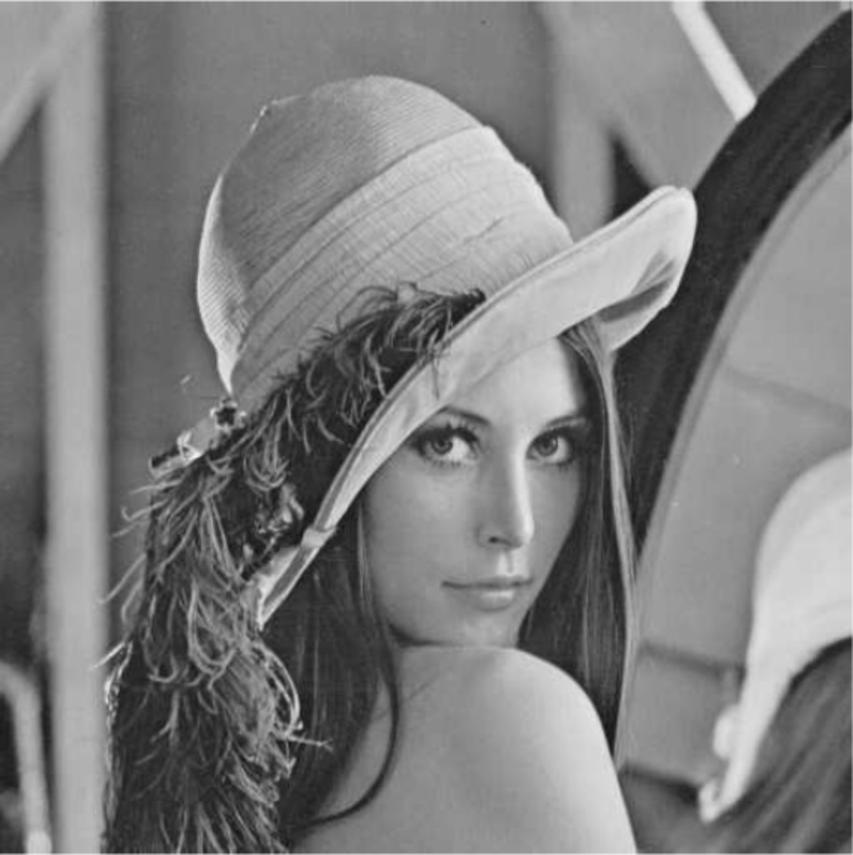
\includegraphics[scale=0.5]{images/lena.pdf} 
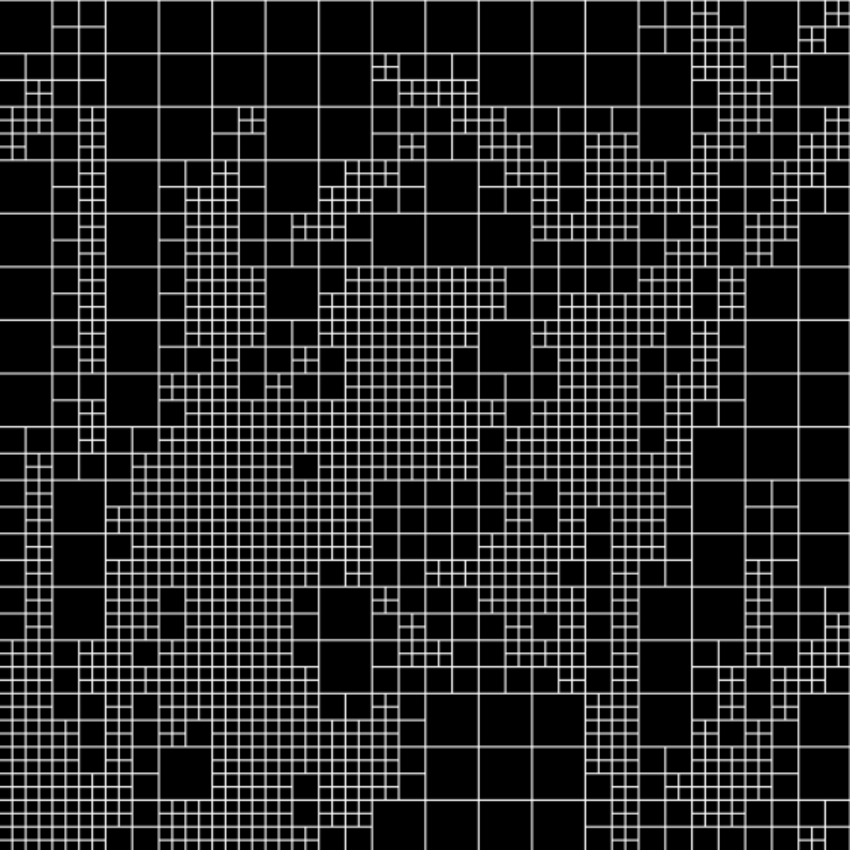
\includegraphics[scale=0.5]{images/quadlena.pdf} 
\caption{Quadtree su Lena, $Q_{\text{min}} = 8$, $Q_{\text{max}} = 64$, $e_c = 0.4$}
\end{figure}

Oltre al partizionamento con \emph{quadtree}, esistono altri metodi applicabili in questo contesto, ad esempio il metodo di partizionamento HV ed il metodo di partizionamento triangolare, che va a generare sottoimmagini non quadrate e può essere quindi vantaggioso nei casi in cui l'immagine di partenza contenga un gran numero di linee oblique (che non sono facilmente coperte da metodi di partizionamento basati su quadrati).

\subsection*{L'algoritmo}

Abbiamo ora a disposizione tutti gli elementi che ci servono per descrivere ad alto livello il funzionamento dell'algoritmo di codifica frattale. Lo riportiamo di seguito:

\begin{framed}
\begin{algorithmic}
\Procedure{Encode}{$e_c$, $r_{\text{min}}$}
\State $R_1 \gets [0,1]^2$
\State $R \gets R \cup R_1$
\State Segna $R_1$ come non coperto
\While{$\exists R_i \in R$ non coperto}
	\State $D_i, w_i \gets$ \Call{bestcover}{$R_i$}  
	\If{$d\big(f \cap (R_i \times I), w_i(f)\big) < e_c$ OR $ \text{size}(R_i) \leq r_{\text{min}}$}
		\State Segna $R_i$ come coperto
		\State $W \gets W \cup w_i$
	\Else	
		\State Partiziona $R_i$ in 4 parti $R_a, R_b R_c, R_d$ 
		\State $R \gets R \setminus R_i$
		\State $R \gets R \cup \{R_a, R_b, R_c, R_d\}$
		\State Segna $R_{\{a,b,c,d\}}$ come non coperti
	\EndIf
\EndWhile
\EndProcedure
\end{algorithmic}
\end{framed}

La procededura \textproc{bestcover} prende come input una sottimmagine $R_i$, e ritorna la sottoimmagine $D_i$ e la rispettiva trasformazione $w_i$ che coprono meglio $R_i$.

\begin{framed}
\begin{algorithmic}
\Procedure{bestcover}{$R_i$}
\State $score \gets \infty$
\State $d, w \gets$, NULL, NULL
\ForAll{$D_i \in D$}
	\State $w_{\text{temp}}, s \gets$ \Call{score}{$D_i, R_i$}
	\If{$s < score$}
		\State $w \gets w_{\text{temp}}$
		\State $score \gets s$
		\State $d \gets D_i$
	\EndIf
\EndFor \\
$~~~~$\Return $d, w$
\EndProcedure
\end{algorithmic}
\end{framed}

La procedura \textproc{score} restituisce una trasformazione $w_i$ ed uno $score$ che indica il livello di somiglianza tra la sottoimmagine di partenza $R_i$ e la sottoimmagine calcolata $D_i$.

\chapter{Aspetti Pratici e implementazione}

In questo capitolo forniamo un'implementazione didattica dell'algoritmo di compressione usando frattali per permettere di comprenderne gli aspetti pratici . Il codice è stato scritto in linguaggio MATLAB ed è possibile scaricarlo da \url{https://github.com/luca-dex/shiny-octo-dubstep}.

\section{Creazione del Dominio}

Il primo passo dell'algoritmo è quello di andare a creare, partendo dall'immagine da comprimere, il dominio $D$. Questa operazione è descritta nel frammento di codice riportato di seguito.

\begin{minted}[linenos=true]{matlab}
function [ d, d2 ] = domains( image, range_sizes, l )
if nargin < 3
    l = 2;
end
d = {1000,2};
dim = length(image);
index = 1;
counter = 1;
range_sizes = sort(range_sizes, 'descend');
for size = range_sizes
    step = size / l;
    for i = 1:step:(dim-size)
        for j = 1:step:(dim-size)
            counter = counter + 1;
            imm = image(i:i+size-1, j:j+size-1);
            if check_equals(d, imm, index-1)
                continue
            end
            d(index,1) = {imm};
            d(index,2) = {[i j size]};
            index = index + 1;
        end
    end
end
\end{minted}

Inizialmente, righe 2-4, viene definito il passo di sovrapposizione tra le immagini del dominio; di default la sovrapposizione è metà della dimensione dell'immagine. Successivamente, riga 10, si itera su ogni dimensione che si vuole assegnare al dominio e per ognuna di si va a definire lo step di sovrapposizione come \texttt{size / l}, riga 11. I passi successivi, righe 12 e 13 sono quello di andare ad individuare tutti gli inizi di sottoimmagine del dominio (angolo in alto a sinistra dell'immagine), dato il valore di \texttt{step}, e quello prendere l'immagine di dimensione \texttt{size}, riga 15. Se questa sottoimmagine non è ancora presente nel dominio, riga 16, allora la si memorizza, riga 19, unitamente alle sue coordinate e alla sua dimensione, riga 20.

A questo punto è abbiamo creato il dominio $D$ che andremo ad utilizzare nei possimi passi dell'algoritmo. Per comodità, siccome durante i confronti ogni immagine nel dominio viene dimezzata, al termine di questa procedura provvediamo a salvare una copia di ogni immagine del dominio di dimensioni dimezzate con opportuna trasformazione lineare.

\section{Encoding}

Ora si cerca di trovare una copertura ottimale per ogni partizione dell'immagine.

\begin{minted}[linenos=true]{matlab}
function [ partial_enc ] = 
    qtfunction(img, pos, size, split_t, min_size, max_size, doms, min_rms)

    global img_copy;
    x = pos(1);
    y = pos(2);
    partial_enc = [];

    if size/2 > max_size
        a = qtfunction(img, [x y], size/2, split_t, 
            min_size, max_size, doms, min_rms);
        b = qtfunction(img, [x+size/2 y], size/2, split_t, 
            min_size, max_size, doms, min_rms);
        c = qtfunction(img, [x y+size/2], size/2, split_t, 
            min_size, max_size, doms, min_rms);
        d = qtfunction(img, [x+size/2 y+size/2], size/2, split_t, 
            min_size, max_size, doms, min_rms);
        partial_enc = [a; b; c; d;];
        return
    end

    rms = repmat(+Inf, [1 4]);
    ts = zeros(1, 4);
    doms_ind = zeros(1, 4);

    for i = 1:length(doms)
        d = doms{i,1};
        if length(d) ~= size/2
            continue
        end
        
        if rms(1) > min_rms
            [r, t] = sup_dist(img(x:(x + size/2 -1), 
                                  y:(y + size/2 -1)), d);
            if r < rms(1)
                rms(1) = r;
                ts(1) = t;
                doms_ind(1) = i;
            end
        end
        
        if rms(2) > min_rms
            [r, t] = sup_dist(img((x + size/2):(x+size-1), 
                                   y:(y + size/2 -1)), d);
            if r < rms(2)
                rms(2) = r;
                ts(2) = t;
                doms_ind(2) = i;
            end
        end
        
        if rms(3) > min_rms
            [r, t] = sup_dist(img(x:(x + size/2 - 1), 
                                 (y + size/2):(y+size-1)), d);
            if r < rms(3)
                rms(3) = r;
                ts(3) = t;
                doms_ind(3) = i;
            end
        end
        
        if rms(4) > min_rms
            [r, t] = sup_dist(img((x + size/2):(x+size-1) , 
                                  (y + size/2):(y+size-1)) , d);
            if r < rms(4)
                rms(4) = r;
                ts(4) = t;
                doms_ind(4) = i;
            end
        end        
    end

    if rms(1) > split_t && size/2 > min_size
        partial_enc = [partial_enc; qtfunction(img, [x y], size/2,
             split_t, min_size, max_size, doms, min_rms)];
    else
        img1 = img(x:(x + size/2 -1), y:(y + size/2 -1));
        [s, o] = least_squared_params(img1, doms{doms_ind(1),1});
        partial_enc = [partial_enc; 
            [x y size/2 doms{doms_ind(1),2} ts(1) s o]];
    end

    if rms(2) > split_t && size/2 > min_size
        partial_enc = [partial_enc; qtfunction(img, [x+size/2 y], size/2, 
            split_t, min_size, max_size, doms, min_rms)];
    else
        img1 = img((x + size/2):(x+size-1), y:(y + size/2 -1));
        [s, o] = least_squared_params(img1, doms{doms_ind(2),1});
        partial_enc = [partial_enc; 
            [x+size/2 y size/2 doms{doms_ind(2),2} ts(2) s o]];
    end

    if rms(3) > split_t && size/2 > min_size
        partial_enc = [partial_enc; qtfunction(img, [x y+size/2], size/2, 
            split_t, min_size, max_size, doms, min_rms)];
    else
        img1 = img(x:(x + size/2 - 1), (y + size/2):(y+size-1));
        [s, o] = least_squared_params(img1, doms{doms_ind(3),1});
        partial_enc = [partial_enc; 
            [x y+size/2 size/2, doms{doms_ind(3),2} ts(3) s o]];
    end

    if rms(4) > split_t && size/2 > min_size
        partial_enc = [partial_enc; qtfunction(img, [x+size/2 y+size/2], size/2, 
            split_t, min_size, max_size, doms, min_rms)];
    else
        img1 = img((x + size/2):(x+size-1) , (y + size/2):(y+size-1));
        [s, o] = least_squared_params(img1, doms{doms_ind(4),1});
        partial_enc = [partial_enc; 
            [x+size/2 y+size/2 size/2, doms{doms_ind(4),2} ts(4) s o]];
    end
end
\end{minted}

Come prima operazione si valuta se il partizionamento produce sottoimmagini sufficientemente piccole, riga 9, e, in caso questo non avvenga, si procede a dividere in 4 parti l'immagine considerata e ad applicare ricorsivamente la procedura, righe 10 - 19. 

Successivamente, per ognuna della quattro sottoimmagini generate tramite il partizionamento con \textit{quadtree}, vengono calcolati i valore della distanza $d$ e della rotazione dell'immagine del dominio. Ad esempio per la sottoimmagine in alto a sinistra la procedura parte col considerare tutti gli elementi del dominio, riga 26, e per ognuno, tramite la funzione \texttt{sup\_dist}, riga 33, verificare se viene trovato un valore di distanza $d$ minore di quelli calcolati fino a quel momento. Per fare questa operazione viene considerata anche ogni possibile roto-traslazione dell'immagine stessa. Se il valore è effettivamente minore, questo viene memorizzato, riga 36, unitamente alle indicazioni sulla rotazione e all'indice di posizione dell'elemento del dominio, righe 37 e 38. Questa operazione viene ripetuta per tutte e quattro le sottoimmagini.

Ora che per ogni sottoimmagine è stata individuata la migliore copertura si passa a verificare se questa effettivamente soddisfafa il valore di threshold voluto e di dimensioni minime. In caso positivo si memorizzano tutti i valori necessari, in caso contrario si applica ricorsivamente la funzione al quarto di immagine. Ad esempio per la sottoimmagine in alto a sinistra la procedura parte con il verificare se le soglie di threshold e dimensione sono rispettate, riga 73, e in caso negativo si riapplica la procedura a questo quarto di immagine, righe 74 e 75. Nel caso in cui i valori di soglia siano rispettati invece si calcolano i valori di \texttt{s} e di \texttt{o}, riga 78, e si memorizza il tutto nella mappa $W$, righe 79 e 80.  Questa operazione viene ripetuta per tutte e quattro le sottoimmagini.

A questo punto l'encoding è terminato, in quanto si ha a disposizione la mappa $W$ che, come abbiamo visto precedentemente, contiene tutte le informazioni che servono per trasformare un immagine qualsiasi nell'immagine di partenza.

\section{Metrica}

Nel precedente frammento di codice è stata introdotta la funzione \texttt{sup\_dist} per il calcolo della distanza tra immagine nel dominio e immagine proveniente dal \textit{quadtree}, di seguito è riportato il funzionamento effettivo di questa funzione, che rispecchia le equazioni viste in precedenza per il calcolo della distanza basandosi sui valori ottimali di $s$ e $o$.

\begin{minted}[linenos=true]{matlab}
function [ rms, transf ] = sup_dist( img1, img2 )
    rms_arr = zeros(1,8);

    for i = 1:8
        rms_arr(i) = dsh(img1, rotate_image(img2, i));
    end

    transf = find(rms_arr - min(rms_arr) == 0, 1);
    rms = rms_arr(transf);
end

function [s, o] = least_squared_params(img1, img2)
    n = length(img1)^2;
    a = single(reshape(img2, [1, n]));
    b = single(reshape(img1, [1, n]));

    s = ( n * dot(a, b) - sum(a)*sum(b) ) / ( n * sum(a.^2) - sum(a)^2 );
    s = min(s, 1);
    o = ( sum(b) - s*sum(a) ) / n;
end

function [ rms ] = dsh(img1, img2)
    [s, o] = least_squared_params(img1, img2);

    n = length(img1)^2;
    a = single(reshape(img2, [1, n]));
    b = single(reshape(img1, [1, n]));

    rms = sqrt(( sum(b.^2) + s * (s*sum(a.^2) - 2*dot(a,b) 
        + 2*o*sum(a)) + o*(n*o - 2*sum(b)) ) / n);
end
\end{minted}

La funzione principale è \texttt{sup\_dist} che si occupa di effettuare il confronto tra la sottoimmagine presa in cosiderazione e tutte le possibili 8 rototraslazioni dell'elemento del dominio, righe 4 - 8. Questa funzione restituisce poi il valore della distanza e la rotazione, rappresentata da una mappa di valori da 1 a 8, righe 10 e 11.

La seconda funzione \texttt{least\_squared\_params} si occupa, date due immagini, di trovare i valori di $s$ e di $o$ secondo le equazioni viste nel precedente capitolo, righe 17 - 19.

La terza funzione, \texttt{dsh} si occupa, date due immagini e calcolati i valori di $s$ e di $o$ tramite la precedente funzione, di calcolare il valore della distanza, righe 29 e 30.

\chapter{Test, benchmarks}

asd

\appendix

\chapter{Tutorial per l'esecuzione del codice sorgente}

In questa appendice daremo una breve descrizione di come utilizzare il codice sorgente con cui sono stati realizzati gli esempi e i bechmarcks utilizzati nei vari capitoli di questo documento. 

Per l'esecuzione del codice MATLAB è necessario che sia installato il plugin \textit{Image Processing Toolbox}\footnote{Maggiori dettagli su \url{http://mathworks.com/products/image/}}.

Per l'esecuzione dei benchmark è necessario che siano installati sul sistema \textit{ImageMagick}\footnote{Maggiori dettagli su \url{http://www.imagemagick.org/}}, libreria per la manipolazione di immagini utilizzata per effettuare la compressione in formato JPEG, e \textit{Fiasco}\footnote{Maggiori dettagli su \url{http://github.com/l-tamas/Fiasco}}, libreria sperimentale per la compressione di immagini utilizzando FIC.

\noindent La prima cosa da fare è clonare il repository che contiene tutti i sorgenti:
\shellcmd{git clone https://github.com/luca-dex/shiny-octo-dubstep}

Il contenuto della cartella è organizzato nel seguente modo:

\begin{itemize}
\item \texttt{src/} Contiene i sorgenti dell'algoritmo implementato in MATLAB
\item \texttt{benchmarks} Contiene gli script per eseguire i benchmarks
\item \texttt{doc/} Contiene il sorgente da cui è stato realizzato questo documento
\item \texttt{workspace/} Contiene esempi di immagini compresse realizzate con l'algoritmo implementato in MATLAB
\item \texttt{images/} Contiene alcune immagini campione utilizzabili con gli algoritmi implementati
\end{itemize}

\section{Implementazione MATLAB}

Il codice MATLAB è progettato per essere eseguito in maniera parallela su una macchina quad-core. La prima parte dell'algoritmo è l'encoding dell'immagine. Tutto il setting dei parametri iniziali avviene all'interno del file \texttt{main.m}. I parametri che è possibile configurare sono:

\begin{itemize}
\item \texttt{im} Path dell'immagine da comprimere, che deve essere quadrata ed in formato BMP
\item \texttt{dom\_range} Dimensione degli elementi che verranno salvati nel dominio. Devono essere divisori della lunghezza del lato dell'immagine
\item \texttt{l} Parametro di sovrapposizione. Il default è 2
\item \texttt{min\_rms} La soglia di errore oltre la quale si accetta la copertura selezionata
\item \texttt{max\_range} La soglia di errore oltre la quale si rifiuta la copertura selezionata e si riapplica quadtree 
\item \texttt{output} Path dell'output dell'algoritmo (workspace MATLAB).
\end{itemize}

Una volta che tutti i parametri sono configurati può essere lanciato l'algoritmo. Il tempo di esecuzione è molto alto, in quanto non sono presenti ottimizzazioni particolari, oltre alla parallelizzazione dell'esecuzione. Consigliamo quindi di non eccedere con la dimensione delle immagini.

Una volta che l'immagine è compressa può essere ricostruita con la funzione \texttt{decode\_all}. Dentro a questa funzione deve essere configurato il parametro \texttt{workspace} con il path del workspace salvato dalla funzione precedente. Questa funzione mostra per prima cosa l'immagine originale e, ogni volta che viene eseguito un click all'interno dell'immagine viene mostrato uno step di ricostruzione.

\section{Benchmark}



\end{document}
